\chapter{Bringing Omniscient Debugging Down to the Database}

\newcommand{\tool}{TAR\-DISP}
\newcommand{\SQLextension}{Back-in-time SQL}
%%Context: Debugging and Back-in-Time
%Finding defects in code is a frequent task for every programmer and is often difficult even with a deep understanding of the system.
%To localize failure causes, they examine involved program entities and distinguish relevant from irrelevant behavior and clean from infected state. 
%However, common symbolic debuggers do not support identification of such infection chains very well because they only provide access to the last point of execution without access to the program history.
%Back-in-time also known as omniscient debuggers simplify the debugging process by making it easier to follow cause-effect chains from the observable failure back to the causing defect~\cite{lewis03:debugging_backwards_in_time}.
%These tools provide full access to past events so that developers can directly experiment with the entire infection chain. 

As we have seen, specialized debugging tools can significantly reduce the time needed to locate a bug.
Consequently, many tools and methods that improve debugging have been developed in the past decades~\cite{wong16:a_survey_on_software}.
However, few of these debugging tools consider an important component of every enterprise application: the database.
Back-in-time debuggers, for example, exist for many object-oriented programming languages, such as Java, C++, or JavaScript~\cite{feldman88:igor_a_system,lewis03:debugging_backwards_in_time,barr16:time-travel_debugging_for_javascriptnode,wong16:a_survey_on_software}.
These languages are typically used in the front-end or application layer of a multi-tier application.

%SQLScript\footnote{SQLScript is a proprietary SQL extension for stored procedures in SAP HANA~\cite{sap16:sap_hana_sqlscript_reference}.}. %hofer_design_2006


The application layer of a multi-tier application can interact with the database in multiple ways.
For object-oriented programming languages, \acp{orm} can abstract from database-specific logic by automatically generating queries and converting all data from and to native objects.
In this scenario, the database is mostly used as a persistent storage of business objects from the application layer.
As already discussed in \cref{sec:enterprise_applications}, "\nameref{sec:enterprise_applications}", 
this is not sufficient for modern applications that handle large amounts of data.

%a database connectors like ODBC or JDBC and 
By using query languages like SQL, the application layer can submit arbitrary queries to the database to store, manipulate or obtain data.
Data-heavy operations can be executed faster by sending them to the database~\cite{plattner15:the_in-memory_revolution_how}, even while the data handling logic remains in the application layer
By using language extensions such as SQL/OLB~\cite{eisenberg98:sqlj_part_0_now}, it is even possible to include database queries as native language elements.

However, not all operations can be expressed in a single query.
When queries are submitted from the application layer, intermediate results have to be passed between application layer and database multiple times.
In big-data applications, where the communication channel between database and application is a strong bottleneck, this pattern must be avoided~\cite{plattner15:the_in-memory_revolution_how}.
Hence, the third approach of handling data-heavy operations is to implement them as stand-alone scripts, also called stored procedures, that, when called from the application, run directly in the database.
This reduces communication overhead between layers and allows the database to apply further optimization, such as reordering queries or choosing when to materialize intermediate results.

Basic debugging support exists for many of these methods and supports forward-in-time debugging and inspecting query results while the program is stopped.
However, there are, to the best of our knowledge, no omniscient debuggers that include the database and support SQL queries or database scripts.

%Database languages like SQLScript, a proprietary language for stored procedures in SAP HANA~\cite{sap16:sap_hana_sqlscript_reference}, 

\tmpStart
%Problem: Back-in-time debugger missing for database-level
This is mainly because of two reasons. 
First, back-in-time debuggers typically create a significant overhead on performance and memory consumption~\cite{lewis03:debugging_backwards_in_time,pothier07:scalable_omniscient_debugging,lienhard08:practical_object-oriented_back-in-time_debugging}.
It seems unfeasible to use a back-in-time debugger on top of a database script that processes billions of records.
Second, current back-in-time debugging concepts cannot handle side-effects outside their system that usually happen in writing operations during INSERT and UPDATE statements. 

%Significance: Especially, in business software much development is based on database scripts. 
Due to high performance requirements of handling big data in business applications, companies like SAP have not only a strong demand to move code closer to data~\cite{plattner15:the_in-memory_revolution_how} but also the need to improve development tools at the database-level. 
As existing tools mostly work on the application level, are limited to specific points in time, or work only on an abstract query plan, developers are often left alone when it comes to debug and understand the results of their queries and stored procedures.
We argue that a back-in-time debugger at the bottom of the technology stack is able to close this gap and can support developers in developing and maintaining their queries more efficiently. 
\tmpEnd

\tmpStart

%Solution
We bring the concept of back-in-time debugging to the database and developed \emph{\tool} as an implementation of our approach.

\begin{itemize}
	\item \emph{\tool} ("Tracing And Recorded Data In Stored Procedures") is a back-in-time debugger for stored procedures which can be installed in the SAP HANA in-memory database and programming platform.
		Using \tool, developers can move freely through the execution time of a stored procedure and inspect control flow, variables, and intermediate results.
	
	\item \emph{\SQLextension} is an extension to SQL allowing developers to submit arbitrary queries against previous states of the database 
		and to compare multiple points in time with one query.
		\tool\ provides a console for developers to submit \SQLextension\ queries which use variables or points in time from the current debug session.

	\item \emph{Very low overhead} when recording run-time data and the efficient querying of past database states allow developers to use \tool\ as the default tool for debugging database scripts even on large data sets.
	
\end{itemize}

We evaluated \tool\ with the help of SAP colleagues who worked on a project called \emph{Point of Sales Explorer}~\cite{plattner15:the_in-memory_revolution_how}, which makes heavy use of stored procedures. 
The interviews indicated that failures in stored procedures can be investigated more efficiently with \tool\ than with other existing database development tools.

\tmpEnd

%\subsubsection{Design Concept}
%pros and cons of post mortem,
%pros and cons of database
%discussion insert only
%final decision
%
%\subsubsection{Prototype: Architecture and Schema}
%figure: architecture
%data schema
%tracing code generation and examples
%
%\subsubsection{BiT SQL}
%
%\subsubsection{-TimeTravel queries}
%
%\subsubsection{-TimeDiff queries}
%
%\subsubsection{Evaluation}

\section{Back-in-Time Debugging in Stored Procedures}

In \cref{sec:omni-debugging}, "\nameref{sec:omni-debugging}", we discussed different approaches for implementing back-in-time capabilities in debuggers.
A snapshot-based debugger records program memory at certain intervals, additionally logging I/O-operations to make program re-execution deterministic when the program accesses external resources.
An omniscient debugger records a full execution trace.
This creates a larger overhead on memory and runtime, but allows the debugger to restore program state from any point in time in a post-mortem analysis.
Hybrid approaches record only the control-flow and partial memory snapshots, recovering the remaining state by re-executing parts of the program.
All approaches have in common that they simulate external resources from the program's perspective, but do not allow developers to inspect the resource itself.

From the debugger's perspective, the database is such an external resource and is therefore not covered by back-in-time features by default.
This is a problem for developers debugging database applications.
To evaluate the correctness of a piece of code, it is usually not enough to only see the result of queries in the program.
Instead, developers need to look into the data and maybe even run their own ad hoc queries to understand whether the program behaves correctly.

When including the database in the execution trace, a back-in-time debugger faces two additional problems:
First, much of the data processing happens outside of the program's scope.
Sometimes, state that has impact on a query's result remains entirely in the database and is practically invisible to the application debugger.
The only way to examine such state is through specific database queries.
Second, the debugger can not easily track changes in the state, because the impact of an insert, update, or delete statement is not reported back to the application in the necessary detail.
This affects determinism when re-executing earlier parts of the program.
With live debugging, sometimes this can be mitigated by resetting the database before restarting the program, but a post-mortem analysis can not easily examine intermediate database states when they have been changed.

In stored procedures, result variables are an additional challenge.
These variables represent the result of a query and can be used in subsequent database statements without havin been fetched into the program
In fact, the database may chose to not materialize intermediate results at all.

\tmpStart
Either way, this increases the amount of invisible state, sometimes only for a few instructions, other times for the entire length of the program.
Furthermore, as trace data usually exceeds program data by orders of magnitude, we expect that tracing the processing of every tuple in a large database is not feasible.

With \tool, we focused on stored procedures because they are executed close to the data and, thus, more efficient in handling large data sets.
This does not limit the general validity of our results, as a debugger for stored procedures faces all of the challenges described above.
\tmpEnd

\subsection{Replaying a Stored Procedure}

An application using a database to manage its state create several problems for debugging tools.
However, giving the debugger direct access to the database can open up new possibilities.

The most immediate advantage is that the database persists state beyond the program execution.
Even post-mortem, the state can be directly accessed by the debugger.
Especially in big-data applications, most operations do not change large parts of the state at once.
Depending on the problem scope and length of the debug session, most of the program state likely remains unchanged.
Knowing that the state will still be available, it can be excluded from the execution trace.

Furthermore, programs that rely on the database for data processing have on fundamental difference compared to other programs:
all instructions handling large data sets (i.e., SQL statements) are declarative.
Instead of providing a concrete algorithm for performing the operation, an SQL statement describe the outcome on an abstract, logical level.
At this level a statement can be analyzed without knowing how it is physically executed.
Even if the database later decides to execute a query using a different query plan, this has no impact for a developer trying to understand the functional correctness of a program.
Thus, there is no need to trace the internals of a query's execution like the processing of an array would have to be traced.
As long as the underlying data does not change, the query results need not be recorded either.
For some purposes it will be helpful to record some meta information, such as the execution time or the number of results, but even this data can be recovered later if needed.

Both advantages can only be exploited if the underlying data does not change.
However, given direct access to the database, the debugger can use it efficiently manage old state, too.
Data is already in a format optimized to be processed by the database and does not need to be transferred into another system this way.
With the ability to restore previous states of the database, 
\tmpStart
all that is needed to reproduce the execution of a stored procedure is a sequence of execution steps.
Each step represents an instruction that has side effects on the database or assigns a value or result set to a variable.
As there is, conceptually, no concurrency in a stored procedure, we can use sequential numbering to track the order of steps.
If applicable, a step has a target name, such as the name of a variable or stored procedure, and a string representation of the value, which can be shown to the user in the debug view.
If the step involves a database statement, we also need a timestamp to be able to reproduce the query.
\tmpEnd

\begin{figure}
	\centering
		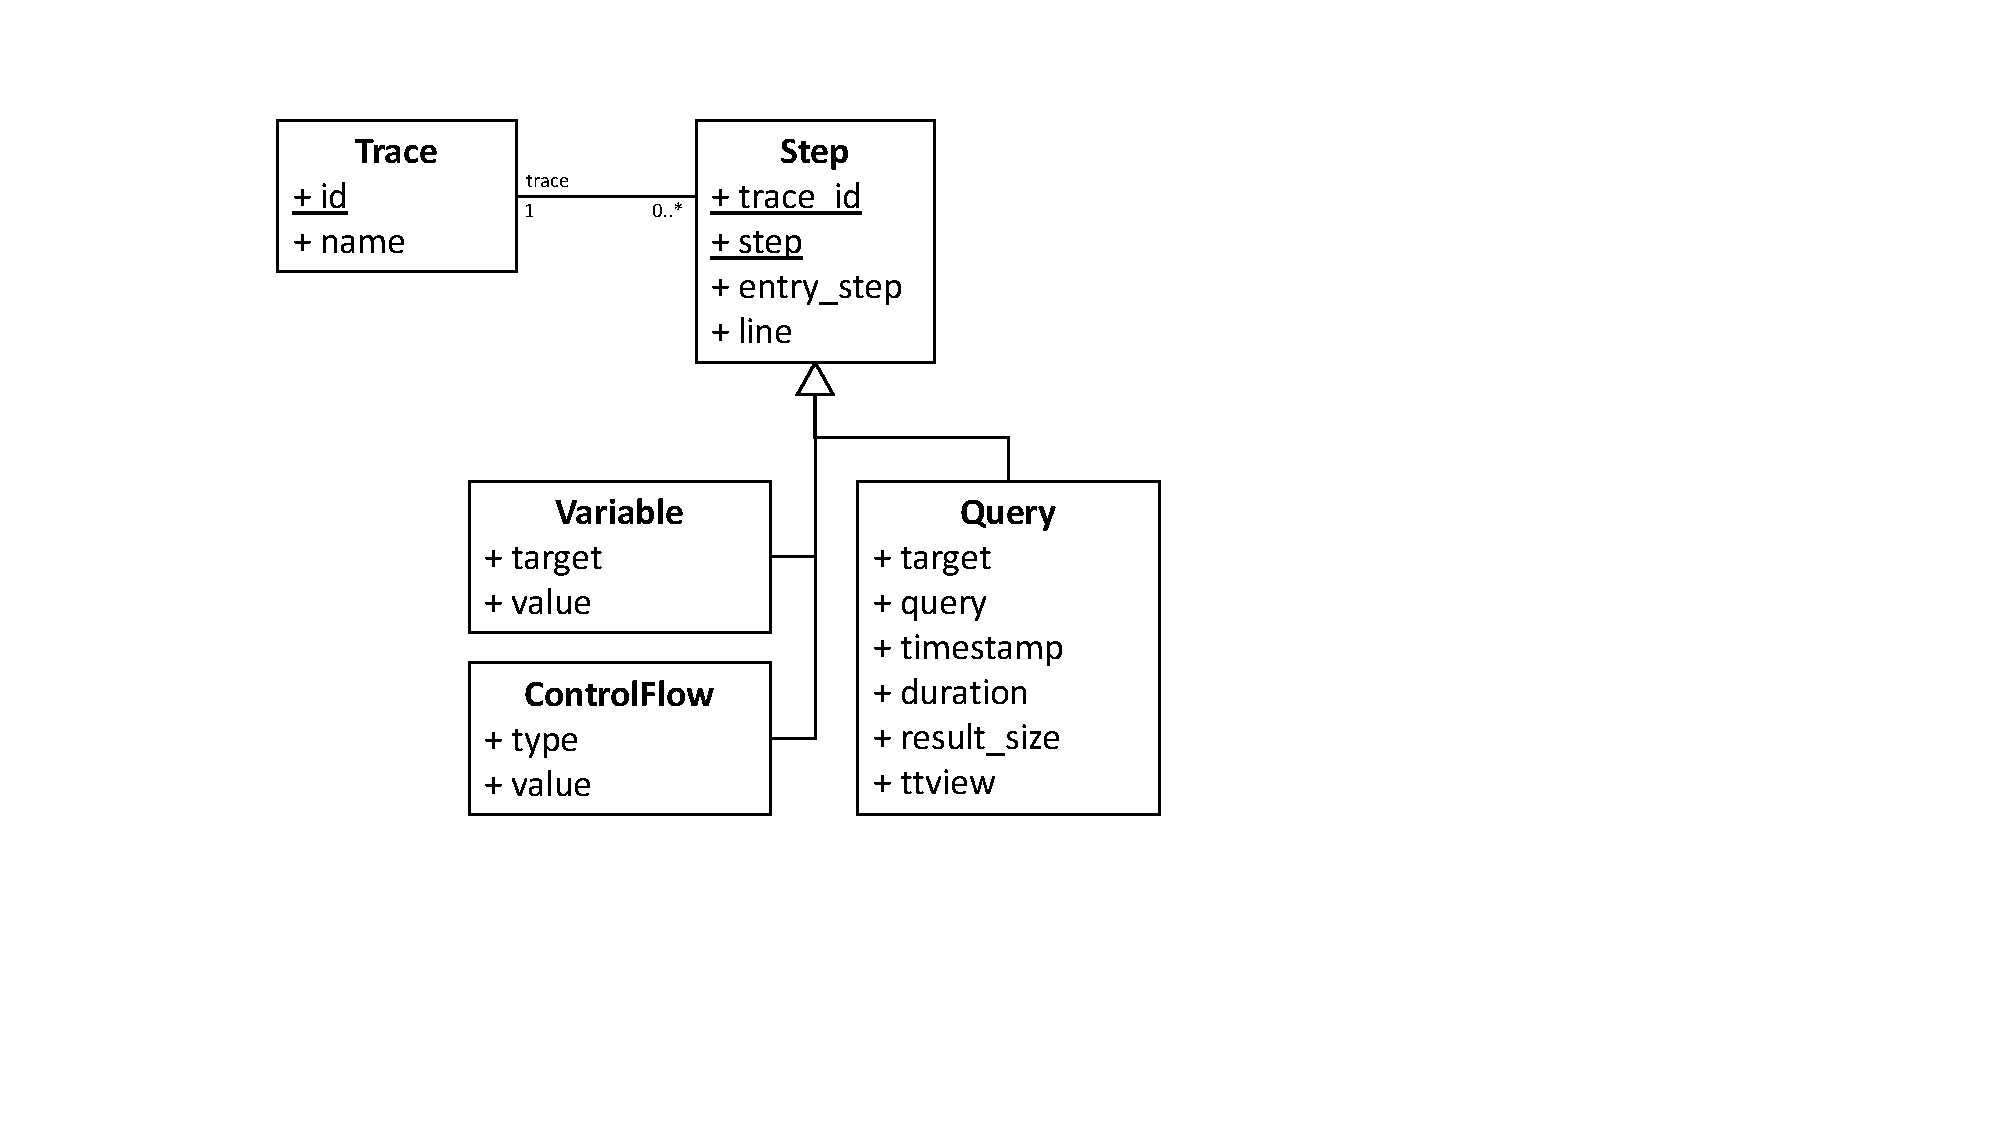
\includegraphics[width=0.9\linewidth]{img/model_sqlodb}
	\caption{Data model of the Stored Procedure debugger.}
	\label{fig:model_odb}
\end{figure}

\Cref{fig:model_odb} shows the relational data model we use to store the required information.
We also explicitly record atomic arguments to each query.
Even though these values can already be derived from the execution trace, storing them explicitly simplifies the process of restoring query results later on.
Furthermore, we record the execution time and the number of rows in the result set for each query.
This information, too, is not strictly needed and can be recovered by re-executing the query.
However, we found that directly providing this information can be helpful to developers, especially for long-running queries.
Lastly, we record the name of a view than can be used to later reproduce the query result.
The view is specifically generated by the debugger, as will be explained in the next subsection.

Because the runtime model of SQLScript is much simpler than that of Java and it was not our goal to create a fully featured debugger for the imperative part of the language, the data model of this debugger is much simpler than that of the Java back-in-time debugger~(\cf \cref{fig:model}, \cpageref{fig:model}), respectively.
This does not limit the general validity of our approach.
The database query as an extra event type could also be added to the Java debugger's trace model and the debugger would handle these queries in just the same way.

\subsection{Reproducing Query Results}

\tmpStart

With the recorded trace data, the debugger has enough information available to replay the execution and to re-execute any query.
However, the query will only yield the same results as long as the underlying data has not changed.

In general, one can expect that debugging will take place on a development machine where no other data manipulation occurs, 
but in cases where this assumption doesn't hold the debugger might end up showing wrong or misleading data the developer.
Furthermore, the debugged stored procedure itself may change the data, which will cause a query to return different results at different points in time.

We ensure consistency over time by following the insert-only approach of our in-memory database.
If we require for all tables that data can never be changed or deleted and annotate all tuples with timestamps of when they have been created and invalidated, we can reconstruct the state of the database of any point in time.
Adding timestamp filters to select queries does not cause a significant slowdown.
Our prototype was built using this approach.
\todo{HANA hat seit neustem "History tables" die das direkt können, wir benutzen aber explizite timestamps weil das momentan noch praktischer ist }

%Thus, SQL queries don't have to be traced at all, although for some purposes it will be helpful to record some meta information, such as the execution time or the number of results.
%\todo{MP: This is not clear to me, yet.}
%Third, the database can be used to efficiently manage old state.
%In-memory databases with insert-only storage automatically retain old data~\cite{plattner09:a_common_database_approach}.
%With insert-only, older versions of the database can be easily reproduced.
%For other databases, insert-only can be achieved by adding validity columns.
%For many business applications, such columns already exist where no data may be deleted for legal reasons.


\subsection{Prototype and Tracing Code Generation}

We developed \tool\ as a prototype implementation of our approach.
Our back-in-time debugger runs in the SAP HANA XS-Engine, a framework for web-applications that is part of the SAP HANA platform.
The user interface is written in HTML5 and JavaScript and queries debugging data via AJAX from the back-end, written in server-side JavaScript.
Traces are stored directly in the database.
Packaged as an XS Application, \tool\ can be directly deployed in a SAP HANA installation.

%With a debugger fully integrated in its database, we would expect the stored procedure execution engine to trace the execution steps.
%However, for our prototype this level of integration was out of scope.\todo{Don't start this way but rather put it into limitation discussion or next steps in summary and than call it producterization}

To be able to trace an execution, we developed a SQLScript pre-processor that parses a stored procedure and adds ´INSERT´ statements around every instruction to collect the required trace data.
To obtain a trace, the debugger then once has to run the traced code instead of the original procedure.
In addition to the tracing code, the pre-processor also generates SQL functions and views that will be used to obtain variable values at given points in time.
For atomic variables, it is simply a search for its most recent step.

For variables containing result tables, a separate view is generated for each query that assigns to that variable.
Each view contains the original code of its query.
Arguments to the query are initialized using their respective views.
On top of that, a master view is generated that chooses the appropriate query view by looking up the requested step in the recorded trace.
%\todo{AT: How much detail?}

\begin{figure}
	\centering
		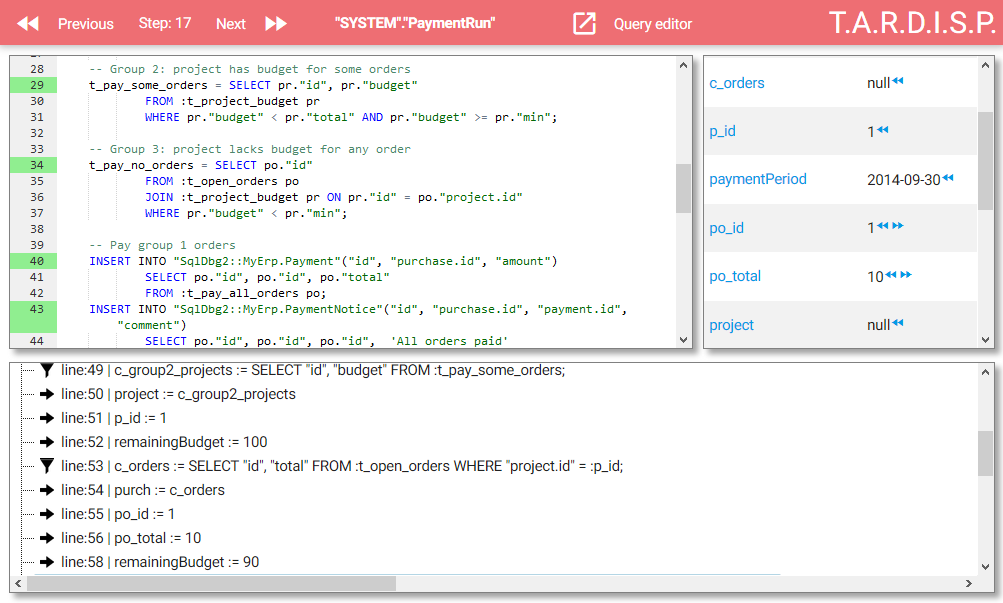
\includegraphics[width=\linewidth]{img/odb.png}
	\caption{User interface of the \tool\ debugger.}
	\label{fig:odb}
\end{figure}

The user interface looks like a typical debugger and is shown in \cref{fig:odb}.
The top-left part of the screen shows the code.
Above, a toolbar contains buttons allowing developers to step forward and backward.
Between the step buttons, the current step number is shown.
Below, \tool\ shows a tree of all execution steps instead of a stack trace.

Next to the code, current variable values are shown.
Arrow buttons allow to jump to the previous or next assignment of the variable.
For variables containing a query result, the size of the result is shown.
Clicking the variable opens a query window that shows the variable's content and allows the developer to submit time-travel queries, which will be explained in the next section.

\section{Back-in-Time SQL}



\newcommand{\red}[1]{\textcolor{DarkRed}{#1}}
\newcommand{\gr}[1]{\textcolor{Green}{#1}}
\newcommand{\timediffresult}{
\begin{table}%
	\begin{tabulary}{\textwidth}{RRRRRRR} \toprule %rlrrrlr
	%pr.id & pr.name 	& pr.budget  & total & po2.id & po2.status & po2.total \\ \midrule
		\multicolumn{3}{c}{pr.} & \multicolumn{1}{c}{po.} & \multicolumn{3}{c}{po2.} \\
	\cmidrule(lr){1-3} \cmidrule(lr){4-4} \cmidrule(lr){5-7}
	~id & name & budget  & total & ~id & status & total \\ \midrule
	
				&					  & \red{1200} & \red{1500} &	  & \red{open} &					\\
	1			& Project 1 & 200			 	 & 500 			  & 1 & paid 			 & 1000			\\
				&						& \gr{-300}  & \gr{0}		  &	  &						 &					\\ \midrule

				&					  & \red{1200} & \red{1500} &	  & 					 &					\\
	1			& Project 1 & 200				 & 500 			  & 2 & open 			 & 500			\\
				&						& \gr{-300}  & \gr{0}		  &	  & \gr{paid}	 &					\\ \bottomrule
	\end{tabulary}
	\caption{Result of a time-diff query, with multiple values in some columns. Red indicates a different value at the \emph{before} step, green indicates a different value at the \emph{after} step.}
	\label{tab:diffresult}
\end{table}
%\ctable[caption={Result of a time-diff query, with multiple values in some columns. Red indicates a different value at the \emph{before} step, green indicates a different value at the \emph{after} step.},label=tab:diffresult,doinside={\small}]
				%{rlrrrlr}{}{
	%pr.id & pr.name 	& pr.budget  & total & po2.id & po2.status & po2.total \ML
	%
				%&					  & \red{1200} & \red{1500} &	  & \red{open} &					\NN
	%1			& Project 1 & 200			 	 & 500 			  & 1 & paid 			 & 1000			\NN
				%&						& \gr{-300}  & \gr{0}		  &	  &						 &					\ML
%
				%&					  & \red{1200} & \red{1500} &	  & 					 &					\NN
	%1			& Project 1 & 200				 & 500 			  & 2 & open 			 & 500			\NN
				%&						& \gr{-300}  & \gr{0}		  &	  & \gr{paid}	 &					\ML
%}
}
%\newcommand{\timediffresult}{
%\ctable[caption={Result of a time-diff query, with multiple values in some columns. Red indicates a different value at the \emph{before} step, green a different value at the \emph{after} step.},label=tab:diffresult,doinside={\small}]
				%{rrrrrrr}{}{
	%\multicolumn{3}{c}{pr.} & \multicolumn{1}{c}{po.} & \multicolumn{3}{c}{po2.} \NN
	%\cmidrule(lr){1-3} \cmidrule(lr){4-4} \cmidrule(lr){5-7}
	%id & name & budget  & total & id & status & total \ML
	%
				%&						& \red{1200} & \red{1500} &	  & \red{open} &					\NN
	%1			&	Project 1	& 200			 	 & 500 			  & 1 & paid 			 & 1000			\NN
				%&						& \gr{-300}  & \gr{0}		  &	  &						 &					\ML
%
				%&						& \red{1200} & \red{1500} &	  & 					 &					\NN
	%1			&	Project 1	& 200				 & 500 			  & 2 & open 			 & 500			\NN
				%&						& \gr{-300}  & \gr{0}		  &	  & \gr{paid}	 &					\ML
%}
%}

\tmpStart

In our setup, the debugger has to recreate intermediate results of a stored procedure.
We generalized this feature to enable developers to submit arbitrary queries against the database of any previous point in time.
Furthermore, we allow developers to compare query results from different points in time and even query for changes in the data.
We defined \SQLextension, a super-set of SQL introducing a new keyword and a new operator.

\subsection{A SQL Clause to Query Points in Time}

As an example, we consider a stored procedure that triggers the payment of purchase orders.
Users reported a bug: projects sometimes exceed their budget, which is not supposed to happen.
Developers might start debugging this issue and the related stored procedure with \tool.
However, they soon realize that the number of projects is too large to continue stepping manually.
Instead, they open \tool's SQL console and submit the query shown in \cref{lst:ttravel} to look into the ´select_projects´ variable, which contains ids, names, and budgets of all projects to be processed.
To better understand the data, they also sum up the total amount of all open purchase orders for each project.

%\Cref{lst:ttravel} shows the query to fetch all selected projects together with the total amount of open orders\todo{The previous paragraph already explains the code - reference to listing needs to be earlier.}.
%We will use it as an example to show how \tool\ handles time-travel queries.

%\begin{figure} % IEEE says put code in figures
%\begin{lstlisting}
\begin{lstlisting}[language=HanaSQL,float,caption={Example for a time-travel query: select the current total of open orders for previously selected projects at step 1623 of the execution},label=lst:ttravel]
  SELECT pr.id, pr.name, pr.budget, SUM(po.total)
  FROM :selected_projects pr
	JOIN PurchaseOrders po ON po.project_id = pr.id
	WHERE po.status = 'open'
	GROUP BY pr.id, pr.name, pr.budget
	^§AT STEP§ 1623^
\end{lstlisting}
%\caption{Example for a time-travel query: select the current total of open orders for previously selected projects}
%\label{lst:ttravel}
%\end{figure}

The last line of \cref{lst:ttravel} contains the ´^AT STEP^´ clause, our extension to SQL that allows developers to explicitly query a specific point in time.
When opening the SQL console, \tool\ automatically provides an ´AT STEP´ clause with the number of the current debug step, ´^1623^´ in this case.
Developers can obtain numbers for other steps from the stepping toolbar or the execution tree. 

When the query is submitted, \tool\ applies two transformations before it is passed to the database.
First, all variables are replaced with their corresponding functions or views that were generated during the pre-processing of the stored procedure.
Each function or view receives the specified step number as an argument to be able to produce the correct value or table.
Second, time-stamp filters on the validity columns are added for all tables that are referenced in the query. 
%Because of SAP HANA's insert-only approach, 
This lets all tables appear exactly as they originally were at the specified point in time.

%In our example,
%\begin{lstlisting}[language={Inline},basicstyle=\ttfamily,numbers=none]
  %po.createdOn < ^1623^ AND (po.validTo IS NULL OR po.validTo > ^1623^)
%\end{lstlisting}
%would be added to the where-clause.

Now, the query can be submitted to the database and the result is subsequently presented to the user.

When developers omit the step number, it is taken from the context of the debug session.
This way, developers can step through the execution and observe how the query result changes over time.

\subsection{Time-diff Queries}

Furthermore, \SQLextension\ provides an easier way to find the origin of changes in the data.
To get a better overview about what happened in a segment of code, developers might want to query multiple points in time at once and see the difference in the query result.
In our example, developers are looking for purchase orders that cause projects to exceed their budget.
Using \tool, they identified three important points in time, which we will call \emph{before}, \emph{now}, and \emph{after}.
\emph{Before} is the step where the stored procedure started processing purchase orders, \emph{now} is the current step, and \emph{after} is the final step of the procedure.

In \cref{lst:tdiff}, the query from above was extended to select individual purchase orders for each project.
In line 10, the at-step clause now specifies all three points in time.
This allows developers to query for changes in the data.

Because the steps are named, they can now be used in the query as time qualifiers.
\SQLextension\ introduces the exclamation mark operator that binds an identifier to a step.
In line 6, it is used to limit the search to projects that will exceed their budget before the stored procedure ends;
in line 7, it is used to filter for purchase orders whose status was or will be changed.

%\begin{figure} % IEEE says put code in figures
%\begin{lstlisting}
\begin{lstlisting}[language=HanaSQL,float=t,caption={Example of a time-diff query: "Select all projects that will go over budget and their respective purchase orders"},label=lst:tdiff]
	SELECT pr.id, pr.name, pr.budget, SUM(po.total), po2.id, po2.status, po2.total
	FROM :selectedProjects pr
	JOIN PurchaseOrders po ON po.project_id = pr.id
	JOIN PurchaseOrders po2 ON po2.project_id = pr.id
	WHERE po.status = 'open'
		AND ^now!^pr.budget > 0 AND ^after!^pr.budget < 0
		AND ^before!^po2.status != ^after!^po2.status
	GROUP BY pr.id, pr.name, pr.budget, 
	         po2.id, po2.status, po2.total
	^§AT STEP§ before=817, now=1623, after=2043^
\end{lstlisting}
%\caption{Example of a time-diff query: "Select all projects that will go over budget and their respective purchase orders"}
%\label{lst:tdiff}
%\end{figure}
\timediffresult
\Cref{tab:diffresult} shows a possible result for this query, with one project that goes over budget and two associated purchases.
The values for budget and total of outstanding payments are shown for each of the three steps.
Of the two purchase orders, the first was already marked as "paid" before the current step, the other is about to be paid.

Analyzing this data, it becomes clear that the payment of the second order is what causes the project budget to become negative.
Developers can now click on the green "paid" value to jump exactly to the point in time where this order is updated, knowing that at this point they are very likely to be close to the defect they are looking for.

To produce this result, the query has to be executed three times, once for each point in time, without the time-specific where-conditions.
The partial results are outer-joined on the primary key attributes, then the time-specific filter conditions are applied.
\tool\ rewrites the query to fit everything into a single select statement, which allows the database to compute the entire result in one request.

%The final query selects all values from each sub-query.
In the user interface, changes in the values are highlighted in as shown in \cref{tab:diffresult}.
If a value changed since the \emph{before} step, the old value is shown in red; if a value will change until the \emph{after} step, the new value is shown in green.
When possible, the tuple creation timestamps are used to allow developers to jump exactly to the point in time where the change occurred.

%Then, to prepare the diffing of the results, they are outer-joined on the primary keys and the time-specific filters are applied.
%For performance reasons, all of this happens inside a single SQL query, as shown in \cref{lst:tdifffinal}.
%The execution of the sub-queries is indicated in \linerefn{lst:tdifffinal}{6, 7, and 10}, the time-specific filters can be found in the Where-condition of \linerefn{lst:tdifffinal}{15 and 16}.

%
%In the UI\todo{Instead of many code listing show the UI (this could also include the code)}, the before and after values are only shown if they differ from the now value.
%Clicking on value allows the developer to jump to the ´UPDATE´ or ´INSERT´ statement that caused the change.


\section{Performance Evaluation and Developer Interviews}

\tmpStart

%\ctable[caption=,label=tab:measure1,doinside={\small},width=\linewidth]
				%{lc>{\raggedleft \arraybackslash}p{1.3cm}RR}{}{
				%&		& Normal run& Run with tracing  & Reproducing the result \ML
	%
			 %&	(a) &	1.27 s		& 1.35 s		& 1.21 s		\NN
%Proc. 1& (b)	&	1.61 s		& 1.74 s		& 1.54 s		\NN
			 %&	(c) &	1.73 s		& 1.85 s		& 1.60 s		\ML
%
			 %&	(a) &	1.24 s		& 1.32 s		& 1.19 s		\NN
%Proc. 2& (b)	&	1.61 s		& 1.72 s		& 1.55 s		\NN
			 %&	(c) &	1.69 s		& 1.80 s		& 1.63 s		\ML
%}

\begin{table}
	\centering
	\begin{tabulary}{\textwidth}{lcRRR}
	\toprule
				&		& Normal run& Run with tracing  & Reproducing the result \\ \midrule
	
			 &	(a) &	1.27 s		& 1.35 s		& 1.21 s		\\
Proc. 1& (b)	&	1.61 s		& 1.74 s		& 1.54 s		\\
			 &	(c) &	1.73 s		& 1.85 s		& 1.60 s		\\ \midrule

			 &	(a) &	1.24 s		& 1.32 s		& 1.19 s		\\
Proc. 2& (b)	&	1.61 s		& 1.72 s		& 1.55 s		\\
			 &	(c) &	1.69 s		& 1.80 s		& 1.63 s		\\ \bottomrule
	\end{tabulary}
	\caption{Average execution time for running a stored procedure without and with tracing and for reproducing its result.}
	\label{tab:measure1}
\end{table}

\begin{table}
	\centering
	\begin{tabulary}{\textwidth}{lcRR}
	\toprule
				&		& Regular query& Time-diff query \\ \midrule
	
			 &	(a) &	1.21 s		& 1.51 s	\\
Query 1& (b)	&	1.74 s		& 2.12 s	\\
			 &	(c) &	1.79 s		& 2.23 s	\\ \midrule

			 &	(a) &	61 ms		&  75 ms	\\
Query 2& (b)	&	81 ms		& 100 ms	\\ 
			 &	(c) &	88 ms		& 109 ms	\\ \bottomrule
	\end{tabulary}
	\caption{Average execution times for queries executed normally or as time-diff query.}
	\label{tab:measure2}
\end{table}

%\ctable[caption={Average execution times for queries executed normally or as time-diff query.},label=tab:measure2,doinside={\small},width=\linewidth]
				%{lcRR}{}{
				%&		& Regular query& Time-diff query \ML
	%
			 %&	(a) &	1.21 s		& 1.51 s	\NN
%Query 1& (b)	&	1.74 s		& 2.12 s	\NN
			 %&	(c) &	1.79 s		& 2.23 s	\ML
%
			 %&	(a) &	61 ms		&  75 ms	\NN
%Query 2& (b)	&	81 ms		& 100 ms	\NN
			 %&	(c) &	88 ms		& 109 ms	\ML
%}

We evaluated our \tool\,debugger on a real-world SAP project that has been developed with one of the largest European retail companies. 
This project is called \emph{Point of Sales Explorer}~\cite{plattner15:the_in-memory_revolution_how} and allows category managers to see a collection of the most important key performance indicators (KPIs) for several thousands of products in a unified dashboard.
Based on more than 2 billion records of point of sales data, this application aggregates on the fly the requested KPIs with the help of SAP HANA and allows users to further refine them by stores, vendors, or products as they like. 
In order to implement flexible requests such as returning the revenue and margin per week of current and last year, this application makes heavy use of SQLScript. 
For that reason, it is a proper candidate to measure performance and interview its developers with respect to our \tool\ tool. 

\subsection{Performance Measurements}

To evaluate the performance of our approach, we deployed \tool\ on a copy of the productive system.
We selected two stored procedures from the Point of Sales Explorer and compared the runtime with and without tracing.
To measure the impact of database size, we ran each procedure with different arguments that would lead to intermediate results of different sizes.
Each value is the average of ten measurements.
%The results are shown in \cref{tab:measure1}.
As \cref{tab:measure1} shows, we found the overhead of tracing to be consistently between six and seven percent.

We also measured the time it takes to reproduce the results of each stored procedure.
This provides us with an upper bound for how long \tool\ would need to compute the value of any variable because in our examples all variables are needed to compute the final result.
The measurements in \cref{tab:measure1} show that reproducing the result is slightly faster than executing the stored procedure.
This was expected because for variables containing atomic values the value could be taken directly from the trace.
Only for variables containing table results, database queries had to be executed again.

Finally, we selected two queries from the stored procedures as examples a developer might submit through the debugger's SQL console and measured their execution time both as a regular query and as a time-diff query.
%Because the Point of Sales Explorer onlyu computes KPIs and does not change the data, we let the time-diff query compare different time-spans of point of sale data\todo{is this disclaimer needed?}.
Again, we used different filter arguments to produce different result sizes.
As \cref{tab:measure2} shows, in each case the runtime overhead of time-diff queries is around 25 percent.

Developers will avoid tools that are too slow to allow fluent working because every delay distracts from the problem to be solved. 
Back-in-time debuggers often suffer from this problem.
Our measurements show that the overhead created by \tool\ is small enough to make it a feasible alternative to existing debugging tools.

\subsection{Interviews}

Besides measuring performance, we also demonstrated our back-in-time debugger to two backend developers of the Point of Sales Explorer. 
These persons have written most of the SQLScript and so know all the challenges when developing close to the database. 
Both had the chance to apply \tool\ in their daily work while we provided tool support and observed them in the background. 
Finally, we have conducted an in-depth interview in order to receive feedback and further improve our tool.

We found out that the main reason for writing SQLScript is to positively influence the optimizer of SAP HANA in order to speed up the overall user request.
If something went wrong at the database-level, the existing tool support was not sufficient. 
The interviewed developers often had to guess why a specific sub-query was not return the expected results. 
%For that reason, they liked our back-in-time debugger and we received a lot of positive feedback.
For this, they liked \tool\ as it could not only show formerly hidden results but also helped them to understand and follow back the reasons behind a failure cause. 
The greatest improvement was reported for debugging stored procedures that take a table of data as an argument, whose cumbersome preparation has to be done only once, using \tool.
Composing such an argument with specific data using the existing tools is cumbersome and has to be redone every time the debug session has to be restarted.
Using \tool, it has to be done only once.
Besides that, both developers wished for some new features such as the ability to define temporary tables for testing code and queries.
With this feedback, we see a strong need for better debugging support at the database-level and are eager to further improve our approach.

%We found out that the main reason for writing SQLScript is to positively influence the optimizer of SAP HANA in order to speed up the overall user request.
%This worked very well as long as the newly written code was free of failures. 
%However, if something went wrong at the database-level, the existing tool support was not sufficient. 
%The interviewed developers often had to guess why a specific sub query was not return the expected results. 
%For that reason, they liked our back-in-time debugger and we received a lot of positive feedback.
%For example, \tool\ could not only show formerly hidden results but also helped them to understand and follow back the reasons behind a failure cause. 
%The greatest improvement was reported for debugging stored procedures that take a table of data as an argument.
%Composing such an argument with specific data using the existing tools is cumbersome and has to be redone every time the debug session has to be restarted.
%Using \tool, it has to be done only once.
%Besides that, both developers also revealed several small failures in our debugger and wished for some new features such as the ability to define temporary tables for testing code and queries.
%With this feedback, we see a strong need for better debugging support at the database-level and are eager to further improve our approach.

%\subsection{Threats to Validity}

\subsection{Limitations}

Our implementation of \SQLextension\ currently has two limitations.

First, time-diff queries can only be executed on tables that have clearly defined primary keys because key attributes are required to track a tuple's version over time.
For a query like "Sum budgets per project category", it has to be clear that categories are the entities that keep their identity over time.
Here, an additional syntax extension could be used to convey this kind of information.

Second, it is currently not possible to use time qualifiers on identifiers outside of the where clause.
We can imagine that there may be a need to use time qualifiers in other SQL clauses, such as the select or order-by clause.
In other use cases, developers might want to attach a time qualifier directly to a table.



\tmpEnd